\documentclass[10pt]{article}
\usepackage{tikz}
\usetikzlibrary{shapes.misc}
\usepackage[margin=0cm]{geometry}
\pagestyle{empty}
\tikzstyle{every node}=[cross out, draw, red]

\begin{document}

\vspace*{\fill}
\begin{center}
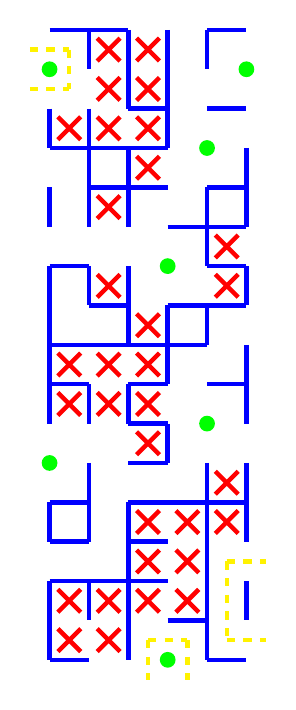
\begin{tikzpicture}[x=0.5cm, y=-0.5cm, ultra thick, blue]
% Walls
    \draw (0,0) -- (2,0);
    \draw (4,0) -- (5,0);
    \draw (2,2) -- (3,2);
    \draw (4,2) -- (5,2);
    \draw (0,3) -- (3,3);
    \draw (1,4) -- (3,4);
    \draw (4,4) -- (5,4);
    \draw (3,5) -- (5,5);
    \draw (0,6) -- (1,6);
    \draw (4,6) -- (5,6);
    \draw (1,7) -- (2,7);
    \draw (3,7) -- (5,7);
    \draw (0,8) -- (4,8);
    \draw (0,9) -- (1,9);
    \draw (2,9) -- (3,9);
    \draw (4,9) -- (5,9);
    \draw (2,10) -- (3,10);
    \draw (2,11) -- (3,11);
    \draw (0,12) -- (1,12);
    \draw (2,12) -- (5,12);
    \draw (0,13) -- (1,13);
    \draw (2,13) -- (3,13);
    \draw (0,14) -- (3,14);
    \draw (3,15) -- (4,15);
    \draw (0,16) -- (1,16);
    \draw (4,16) -- (5,16);
    \draw (0,2) -- (0,3);
    \draw (0,4) -- (0,5);
    \draw (0,6) -- (0,10);
    \draw (0,12) -- (0,13);
    \draw (0,14) -- (0,16);
    \draw (1,0) -- (1,1);
    \draw (1,2) -- (1,5);
    \draw (1,6) -- (1,7);
    \draw (1,9) -- (1,10);
    \draw (1,11) -- (1,13);
    \draw (1,14) -- (1,15);
    \draw (2,0) -- (2,2);
    \draw (2,3) -- (2,5);
    \draw (2,6) -- (2,8);
    \draw (2,9) -- (2,10);
    \draw (2,12) -- (2,16);
    \draw (3,0) -- (3,3);
    \draw (3,7) -- (3,9);
    \draw (3,10) -- (3,11);
    \draw (4,0) -- (4,1);
    \draw (4,4) -- (4,6);
    \draw (4,7) -- (4,8);
    \draw (4,11) -- (4,16);
    \draw (5,3) -- (5,5);
    \draw (5,6) -- (5,7);
    \draw (5,8) -- (5,10);
    \draw (5,11) -- (5,13);
    \draw (5,14) -- (5,15);
% Pillars
    \fill[green] (0,1) circle(0.2);
    \fill[green] (5,1) circle(0.2);
    \fill[green] (4,3) circle(0.2);
    \fill[green] (3,6) circle(0.2);
    \fill[green] (4,10) circle(0.2);
    \fill[green] (0,11) circle(0.2);
    \fill[green] (3,16) circle(0.2);
% Inner points in accessible cul-de-sacs
    \node at (1.5,0.5) {};
    \node at (2.5,0.5) {};
    \node at (1.5,1.5) {};
    \node at (2.5,1.5) {};
    \node at (0.5,2.5) {};
    \node at (1.5,2.5) {};
    \node at (2.5,2.5) {};
    \node at (2.5,3.5) {};
    \node at (1.5,4.5) {};
    \node at (4.5,5.5) {};
    \node at (1.5,6.5) {};
    \node at (4.5,6.5) {};
    \node at (2.5,7.5) {};
    \node at (0.5,8.5) {};
    \node at (1.5,8.5) {};
    \node at (2.5,8.5) {};
    \node at (0.5,9.5) {};
    \node at (1.5,9.5) {};
    \node at (2.5,9.5) {};
    \node at (2.5,10.5) {};
    \node at (4.5,11.5) {};
    \node at (2.5,12.5) {};
    \node at (3.5,12.5) {};
    \node at (4.5,12.5) {};
    \node at (2.5,13.5) {};
    \node at (3.5,13.5) {};
    \node at (0.5,14.5) {};
    \node at (1.5,14.5) {};
    \node at (2.5,14.5) {};
    \node at (3.5,14.5) {};
    \node at (0.5,15.5) {};
    \node at (1.5,15.5) {};
% Entry-exit paths without intersections
    \draw[dashed, yellow] (-0.5,0.5) -- (0.5,0.5);
    \draw[dashed, yellow] (-0.5,1.5) -- (0.5,1.5);
    \draw[dashed, yellow] (4.5,13.5) -- (5.5,13.5);
    \draw[dashed, yellow] (2.5,15.5) -- (3.5,15.5);
    \draw[dashed, yellow] (4.5,15.5) -- (5.5,15.5);
    \draw[dashed, yellow] (0.5,0.5) -- (0.5,1.5);
    \draw[dashed, yellow] (2.5,15.5) -- (2.5,16.5);
    \draw[dashed, yellow] (3.5,15.5) -- (3.5,16.5);
    \draw[dashed, yellow] (4.5,13.5) -- (4.5,15.5);
\end{tikzpicture}
\end{center}
\vspace*{\fill}

\end{document}
